\pdfoptionpdfminorversion=5
\documentclass[9pt,hyperref={pdfpagelabels=false}]{beamer}

\mode<presentation> {
    \usetheme{HHUD}
    \setbeamercovered{invisible}
}
\usepackage[ngerman]{babel}
\usepackage[utf8x]{inputenc}
\usepackage{times}
\usepackage[T1]{fontenc}
\usepackage{amsmath}
\usepackage{subfigure}
\usepackage{graphicx}
\usepackage{hyperref}
\usepackage{grffile}
\usepackage{xmpmulti}
\usepackage{multicol}
\usepackage{appendixnumberbeamer}

% background image
\usebackgroundtemplate{\includegraphics[width=\paperwidth]{fig/background}}
% commands for low and high decoration in frame foot
\newcommand{\footdecorationlow}{\usebackgroundtemplate{\includegraphics[width=\paperwidth]{fig/background_small}}}
\newcommand{\footdecorationhigh}{\usebackgroundtemplate{\includegraphics[width=\paperwidth]{fig/background}}}

\AtBeginSection[] {
  \footdecorationhigh
  \begin{frame}<beamer>
    \thispagestyle{empty}
    \frametitle{Gliederung}
    \vspace{-5mm}
    \tableofcontents[currentsection]
  \end{frame}
  \footdecorationlow
}

\newcommand{\simtd}{$\text{sim}^\text{TD}$}
 
% % % % % % % % % %  CHANGE TOPIC AND AUTHOR INFORMATION HERE % % % % % % % % %
\title[Kurztitel]{A Real-time Streaming Protocol for Large-scale Peer-to-Peer Networks}
\author[Kurzautor]{Christopher Probst}
\institute{Institut für Informatik\\Rechnernetze und Kommunikationssysteme\\Heinrich-Heine-Universität Düsseldorf}
\subject{Informatik}
\date{3.12.2014}
% % % % % % % % % % % % % % % % % % % % % % % % % % % % % % % % % % % % % % % %

\begin{document}

  \footdecorationhigh
  \begin{frame}
    \thispagestyle{empty}
    \titlepage
  \end{frame}
  
  \begin{frame}
    \thispagestyle{empty}
    \frametitle{Gliederung}
    \vspace{-5mm}
    \tableofcontents
  \end{frame}
  \footdecorationlow

  \section{Einleitung}

\begin{frame}
  \frametitle{Motivation}  
  \begin{itemize}
    \item Problem: Datenverbreitung mit Client\,/\,Server Architektur skaliert nicht
    \vspace{1mm}
    \begin{itemize}
      \item Jeder Client erhöht die Auslastung
      \vspace{1mm}
      \item Uploadbandbreite des Servers ist limitiert        
      \vspace{1mm}
      \item Uploadbandbreite der Clients ungenutzt
    \end{itemize}

    \vspace{2mm}

    \item Lösungsansatz: Verwendung eines Peer-to-Peer Netzwerks
    \vspace{1mm}
    \begin{itemize}
      \item Jeder Peer hilft bei der Datenverbreitung
      \vspace{1mm}
      \item Server heißt nun Super-Peer (Peer mit vollständigem Datensatz)
      \vspace{1mm}
      \item Super-Peer und Peers werden gleichmäßig ausgelastet
      \vspace{1mm}
      \item Super-Peer kann Daten trotz geringer Uploadbandbreite schnell verbreiten
    \end{itemize}    
  \end{itemize}
\end{frame}


\begin{frame}
  \frametitle{Zielsetzung}
    Implementierung einer Peer-to-Peer Anwendung zur Verbreitung von Daten:
    \vspace{1mm}
    \begin{itemize}
      \item Uploadbandbreite der Peers effizient nutzen
      \item Zeitpunkt für den Erhalt der Daten bei allen Peers gleich
      \item Gesamtdauer unabhängig von der Anzahl der Peers
      \item Gesamtdauer kleiner als $2 * T_0$.
    \end{itemize}
\end{frame}

  \section{Umsetzung}


\begin{frame}
  \frametitle{Ansatz: Chunked-Swarm}
  Super-Peer teilt die Daten vor dem Transfer in kleine Teile (Chunks):
  \vspace{1mm}
  \begin{itemize}  
    \item Mindestens so viele Chunks wie Peers
    \item Peers beantragen disjunkte Chunks vom Super-Peer
    \item Peers tauschen Chunks untereinander aus
    \item Vereinfachung: Alle Peers haben die gleiche Uploadbandbreite
  \end{itemize} 
\end{frame}


\begin{frame}
  \frametitle{Chunked-Swarm: Ablauf}
  Beispiel: Genauso viele Chunks wie Peers
  \begin{exampleblock}{Phasen}  
    \begin{itemize}
      \item Phase 1 (links): Peers bekommen disjunkten Chunk vom Super-Peer
      \item Phase 2 (rechts): Peers tauschen ihre Chunks untereinander 
    \end{itemize}
  \end{exampleblock}
  \begin{center}
    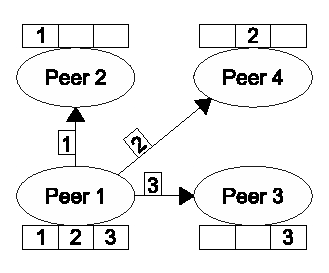
\includegraphics[width=0.4\textwidth]{fig/chunkedswarmmodel1.eps}
    \hspace{0.15\textwidth}
    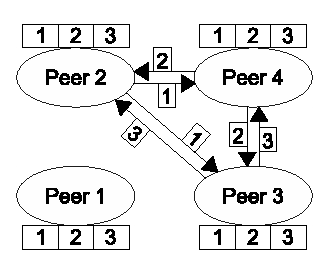
\includegraphics[width=0.4\textwidth]{fig/chunkedswarmmodel2.eps}
  \end{center}
\end{frame}


\begin{frame}
  \frametitle{Chunked-Swarm: Gesamtdauer}
  Beispiel: Genauso viele Chunks wie Peers
  \begin{exampleblock}{Zeitlicher Ablauf}
    \begin{itemize}
      \item Bis $T_0$: Super-Peer 1 schickt disjunkten Chunk an jeden Peer
      \item Ab $T_0$: Jeder Peer schickt Chunk an die anderen beiden Peers
      \item Ab $T_0 + \frac{2}{3} * T_0$: Daten wurden vollständig verbreitet
    \end{itemize}
  \end{exampleblock}
  \begin{center}
    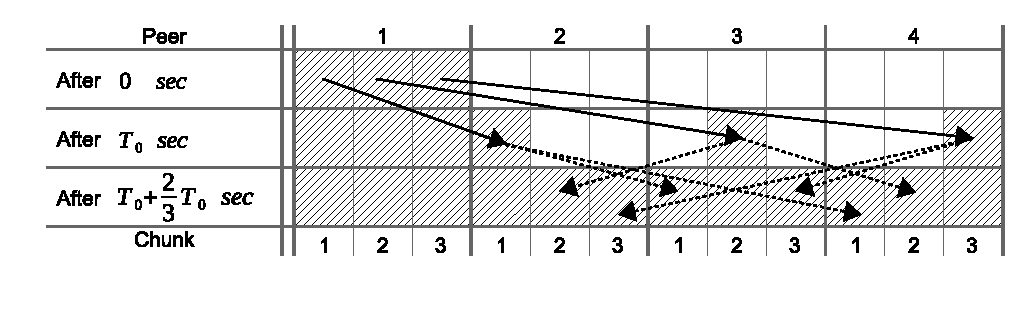
\includegraphics[width=1\textwidth]{fig/chunkedswarmformula1.eps}
  \end{center}
\end{frame}


\begin{frame}
  \frametitle{Chunked-Swarm: Gesamtdauer}
  \begin{block}{Eigenschaften}
    \begin{itemize}  
      \item Verdoppelung der Chunks halbiert die Zeit zwischen $T_0$ und Ende
      \vspace{2mm}
      \item Gesamtdauer: $T(n, c) = T_0\:+\:\frac{n}{c}\:*\:\frac{n-1}{n}\:*\:T_0$, $n \in \mathbb{N}_1$, $c = n\:*\:2^i, i \in \mathbb{N}_0$
      \vspace{2mm}
      \item Real-time: Gesamtdauer immer unter $2 * T_0$
    \end{itemize}
  \end{block}
\end{frame}


\begin{frame}
  \frametitle{Implementierung}
  \begin{itemize}  
    \item Mesh Topologie: Alle Peers sind miteinander verbunden
    \vspace{1mm}
    \item Pull-Based: Chunks werden nur auf Wunsch übertragen
    \vspace{1mm}
    \item Announcements: Jeder Peer kündigt seine Chunks an
    \vspace{1mm}
    \item Traffic-Shaping: Up-/Downloadbandbreite präzise drosselbar
    \vspace{1mm}
    \item Implementiert in Java mit Netty5
  \end{itemize} 
\end{frame}




  \section{Evaluation}

\begin{frame}
  \frametitle{Methodik}
  \begin{itemize}  
  	\item Verschiedene Szenarios
  	\vspace{1mm}
    \item Ein Default-Szenario: Übrige Szenarios sind Abwandlungen
    \vspace{1mm}
    \item Jedes Szenario läuft 10 mal
    \vspace{1mm}
    \item Plots: Durchschnitt und Konfidenzintervall (Konfidenzniveau 95\%)
  \end{itemize}	
\end{frame}



\begin{frame}
  \frametitle{Methodik}
  \begin{block}{Besonderheiten}
    \begin{itemize}
      \item Verbindungen nur virtuell: Kein TCP
      \vspace{2mm}
      \item Keine (De-)Serialisierung von Paketen: Spart CPU und RAM
      \vspace{2mm}
      \item Aber: Paketgröße wird simuliert!
    \end{itemize}
  \end{block}
\end{frame}


%%%
%%% DEFAULT SCENARIO 1
%%%

\begin{frame}
  \frametitle{Default Szenario}
  \begin{block}{Einstellungen}
	  \begin{itemize}  
	    \item 1 Super-Peer und 63 Peers
	    \vspace{2mm}
	    \item Doppelt so viele Chunks wie Peers (126 Chunks)
	    \vspace{2mm}
	    \item Gleiche Uploadbandbreite für Super-Peer und Peers
	    \vspace{2mm}
	    \item Datengröße so gewählt, dass $T_0=10$ Minuten gilt 
	  \end{itemize}		
  \end{block}
\end{frame}


\begin{frame}
  \frametitle{Default Szenario - Completion}
  \begin{itemize}  
    \item Links: Ablauf des Datentransfers
    \item Rechts: Peers absteigend sortiert nach Gesamtdauer
  \end{itemize}

  \begin{center}
    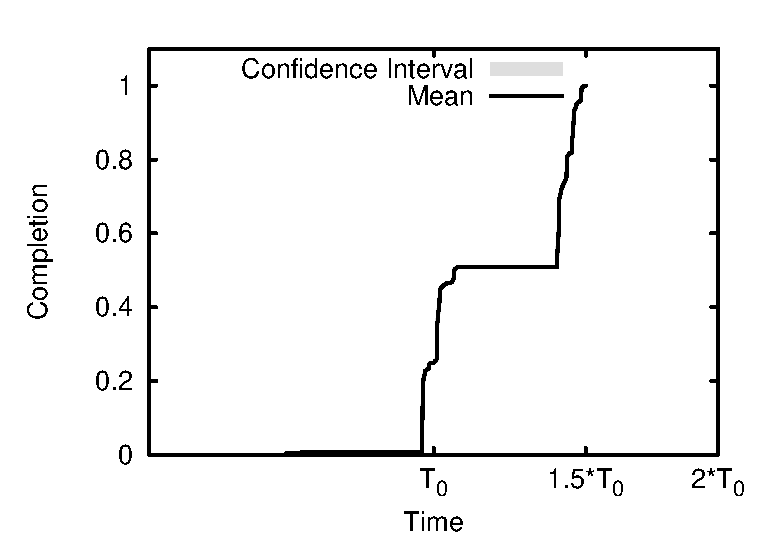
\includegraphics[width=0.49\textwidth]{fig/plots/scenario_1_default/plots/GeneratedMeanChunkCompletion.csv.eps}
    \hfill
    \includegraphics[width=0.49\textwidth]{fig/plots/scenario_1_default/plots/GeneratedMeanSortedChunkCompletion.csv.eps}
  \end{center}
\end{frame}


\begin{frame}
  \frametitle{Default Szenario - Upload/Download}
  \begin{center}
    \includegraphics[width=0.49\textwidth]{fig/plots/scenario_1_default/plots/GeneratedMeanCurrentUploadBandwidth.csv.eps}
    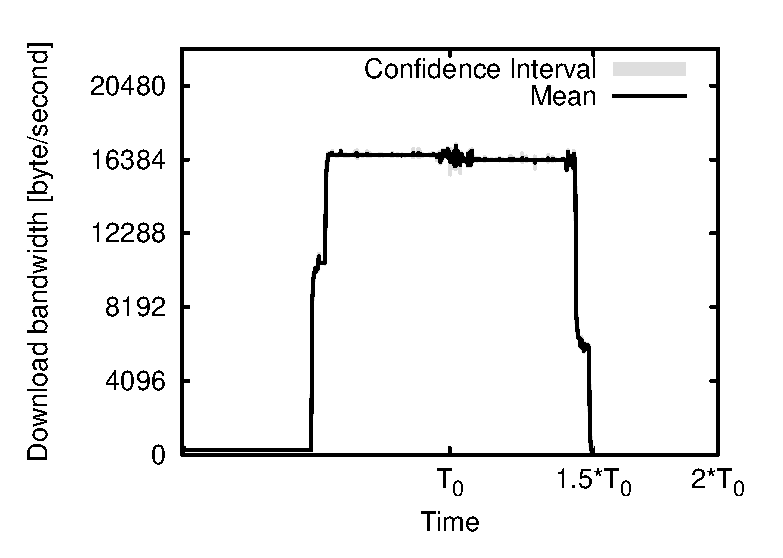
\includegraphics[width=0.49\textwidth]{fig/plots/scenario_1_default/plots/GeneratedMeanCurrentDownloadBandwidth.csv.eps}
  \end{center}
\end{frame}


\begin{frame}
  \frametitle{Default Szenario - Super-Peer Upload}
  \begin{center}
    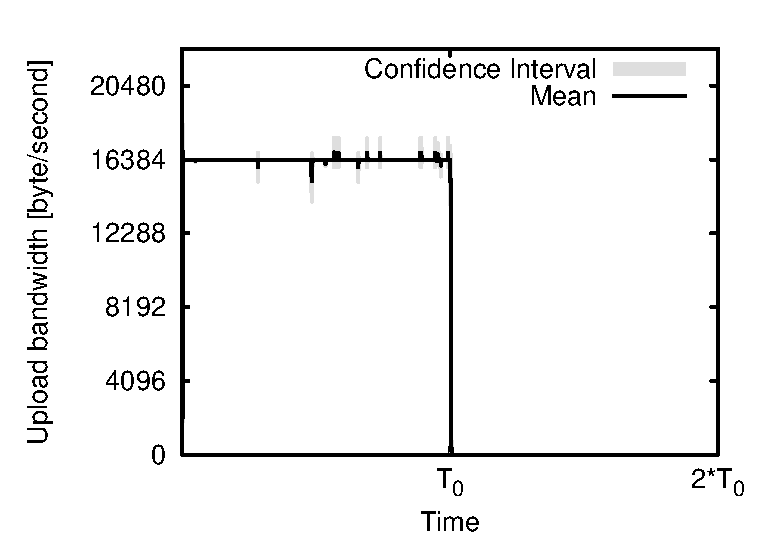
\includegraphics[width=0.49\textwidth]{fig/plots/scenario_1_default/plots/GeneratedMeanCurrentSuperSeederUploadBandwidth.csv.eps}
  \end{center}
\end{frame}

%%%
%%% SCENARIO 128
%%%

\begin{frame}
  \frametitle{Default Szenario mit 128 Peers - Completion}
  \begin{itemize}  
    \item Links: Ablauf des Datentransfers
    \item Rechts: Peers absteigend sortiert nach Gesamtdauer
  \end{itemize}

  \begin{center}
    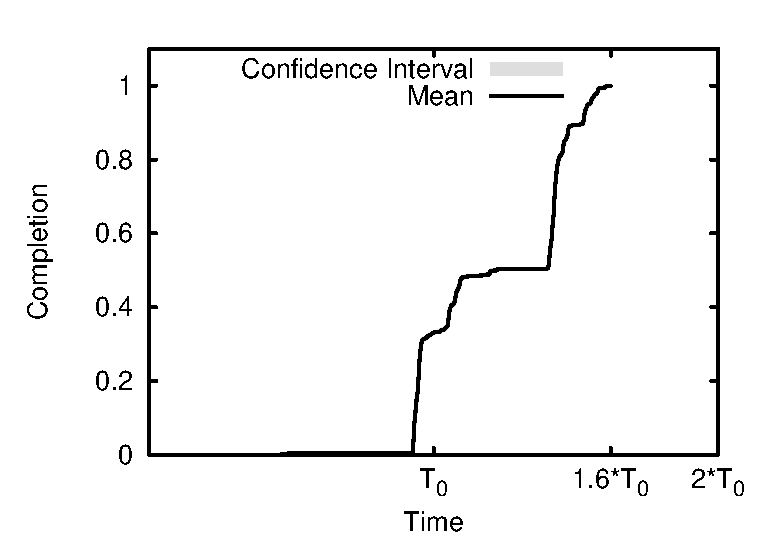
\includegraphics[width=0.49\textwidth]{fig/plots/scenario_4_peer_count_128/plots/GeneratedMeanChunkCompletion.csv.eps}
    \hfill
    \includegraphics[width=0.49\textwidth]{fig/plots/scenario_4_peer_count_128/plots/GeneratedMeanSortedChunkCompletion.csv.eps}
  \end{center}
\end{frame}


\begin{frame}
  \frametitle{Default Szenario mit 128 Peers - Upload/Download}
  \begin{center}
    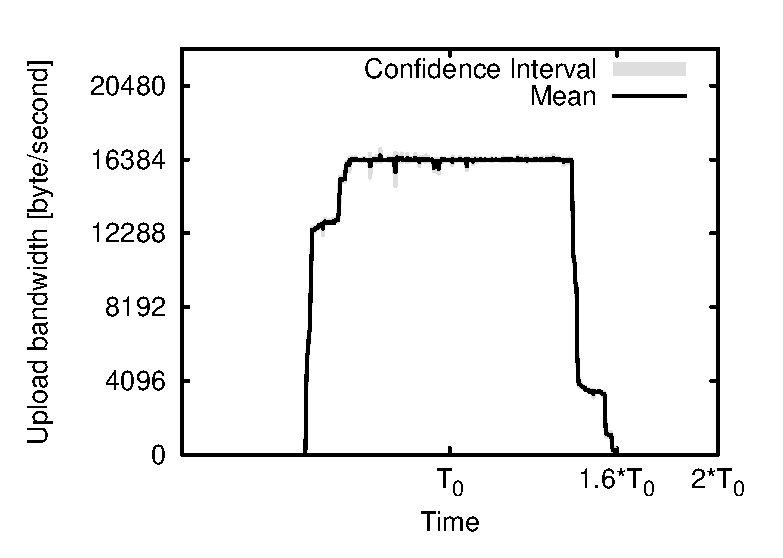
\includegraphics[width=0.49\textwidth]{fig/plots/scenario_4_peer_count_128/plots/GeneratedMeanCurrentUploadBandwidth.csv.eps}
    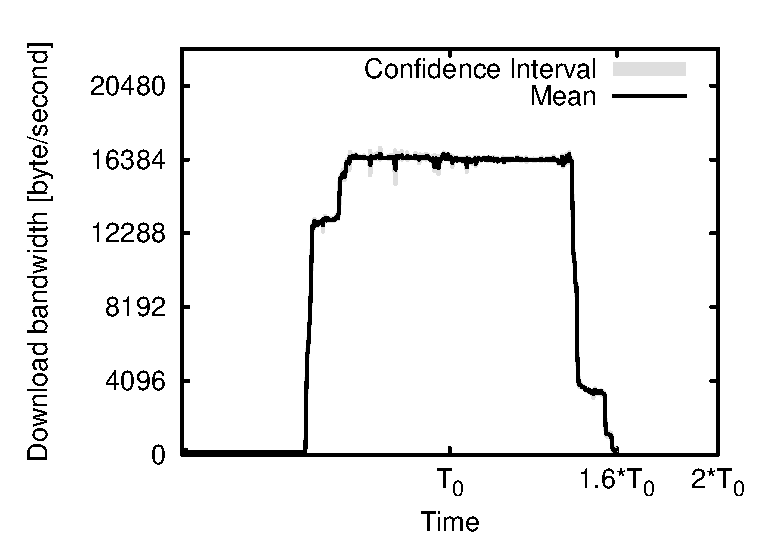
\includegraphics[width=0.49\textwidth]{fig/plots/scenario_4_peer_count_128/plots/GeneratedMeanCurrentDownloadBandwidth.csv.eps}
  \end{center}
\end{frame}


\begin{frame}
  \frametitle{Default Szenario mit 128 Peers - Super-Peer Upload}
  \begin{center}
    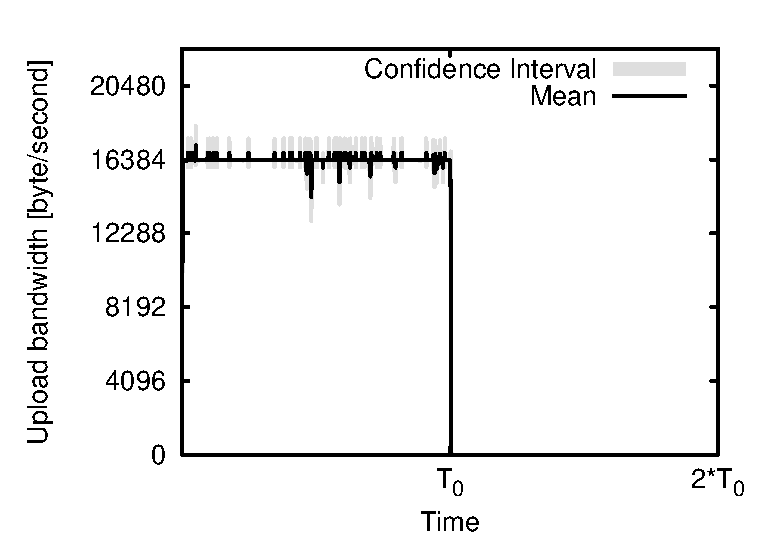
\includegraphics[width=0.49\textwidth]{fig/plots/scenario_4_peer_count_128/plots/GeneratedMeanCurrentSuperSeederUploadBandwidth.csv.eps}
  \end{center}
\end{frame}

%%%
%%% SCENARIO 4x Chunks
%%%

\begin{frame}
  \frametitle{Default Szenario mit 4x Chunkanzahl - Completion}
  \begin{itemize}  
    \item Links: Ablauf des Datentransfers
    \item Rechts: Peers absteigend sortiert nach Gesamtdauer
  \end{itemize}

  \begin{center}
    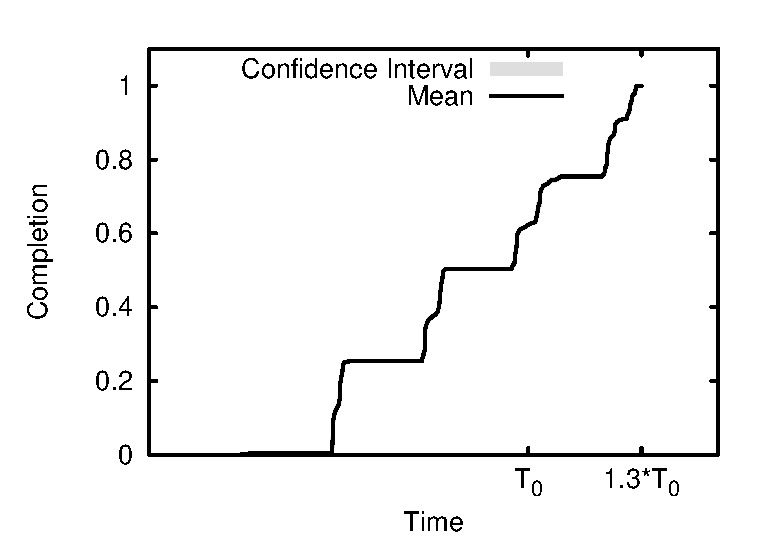
\includegraphics[width=0.49\textwidth]{fig/plots/scenario_15_chunk_count_fac_4/plots/GeneratedMeanChunkCompletion.csv.eps}
    \hfill
    \includegraphics[width=0.49\textwidth]{fig/plots/scenario_15_chunk_count_fac_4/plots/GeneratedMeanSortedChunkCompletion.csv.eps}
  \end{center}
\end{frame}


\begin{frame}
  \frametitle{Default Szenario mit 4x Chunkanzahl - Upload/Download}
  \begin{center}
    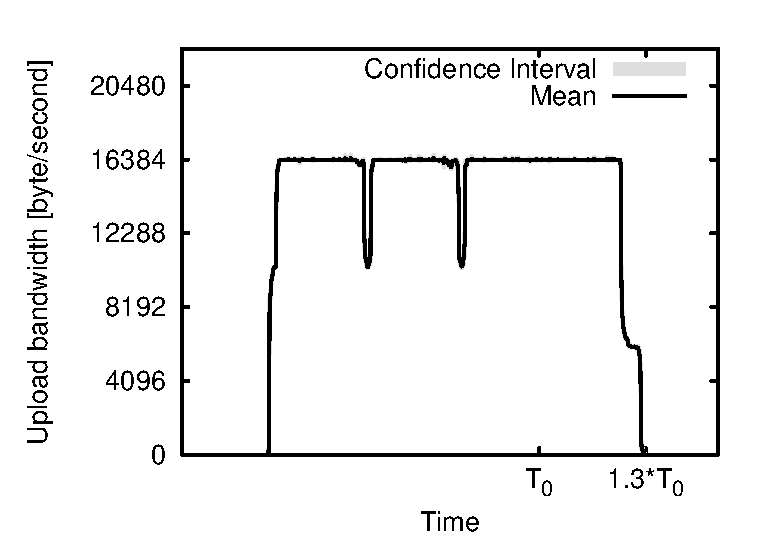
\includegraphics[width=0.49\textwidth]{fig/plots/scenario_15_chunk_count_fac_4/plots/GeneratedMeanCurrentUploadBandwidth.csv.eps}
    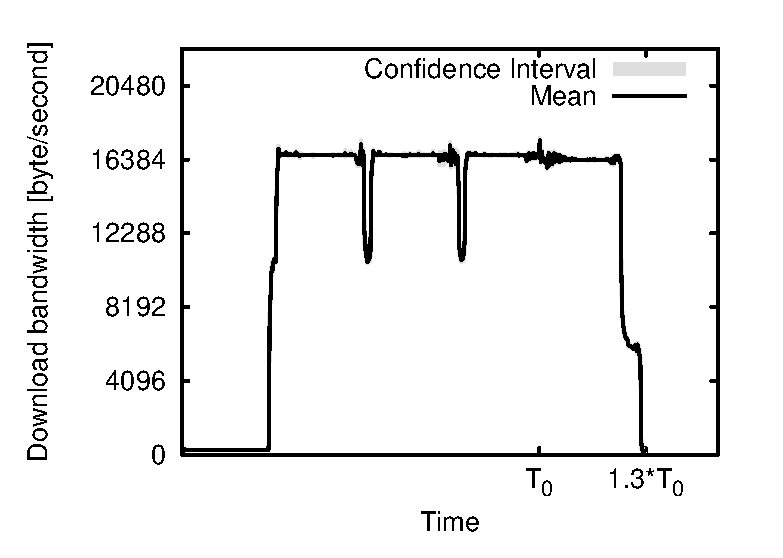
\includegraphics[width=0.49\textwidth]{fig/plots/scenario_15_chunk_count_fac_4/plots/GeneratedMeanCurrentDownloadBandwidth.csv.eps}
  \end{center}
\end{frame}


\begin{frame}
  \frametitle{Default Szenario mit 4x Chunkanzahl - Super-Peer Upload}
  \begin{center}
    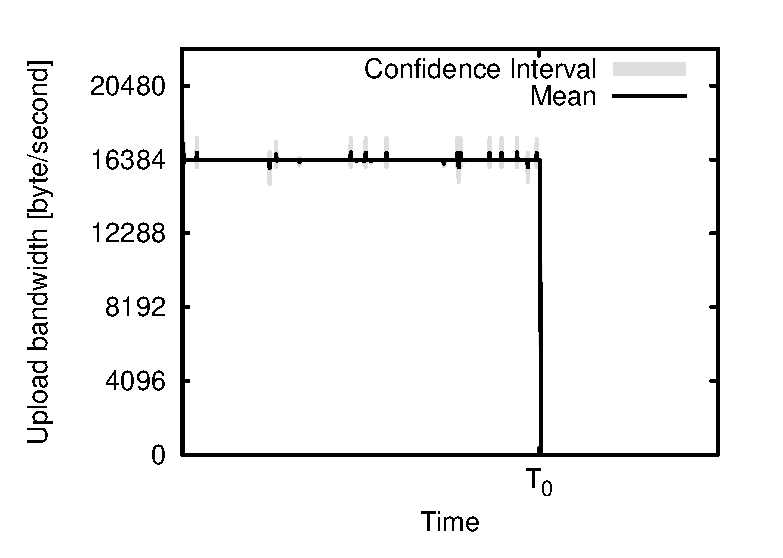
\includegraphics[width=0.49\textwidth]{fig/plots/scenario_15_chunk_count_fac_4/plots/GeneratedMeanCurrentSuperSeederUploadBandwidth.csv.eps}
  \end{center}
\end{frame}


%%%
%%% SCENARIO Parts 20
%%%

\begin{frame}
  \frametitle{Default Szenario mit 20 Datensätzen}
  \begin{block}{Einstellungen}
	  \begin{itemize}  
	    \item Gesamter Datensatz wird in 20 Sub-Datensätze geteilt
	    \vspace{2mm}
	    \item Jeder Sub-Datensatz hat doppelt soviele Chunks wie Peers
	    \vspace{2mm}
	    \item Sub-Datensätze durchnummeriert mit IDs: Kleine IDs zuerst
	    \vspace{2mm}
	    \item Streaming!
	  \end{itemize}		
  \end{block}
\end{frame}

\begin{frame}
  \frametitle{Default Szenario mit 20 Datensätzen - Completion}
  \begin{itemize}  
    \item Links: Ablauf des Datentransfers
    \item Rechts: Peers absteigend sortiert nach Gesamtdauer
  \end{itemize}

  \begin{center}
    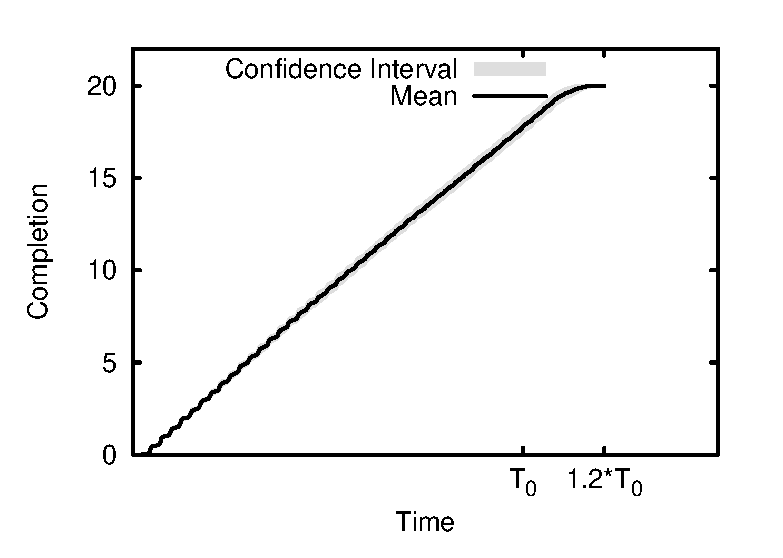
\includegraphics[width=0.49\textwidth]{fig/plots/scenario_6_parts_20/plots/GeneratedMeanChunkCompletion.csv.eps}
    \hfill
    \includegraphics[width=0.49\textwidth]{fig/plots/scenario_6_parts_20/plots/GeneratedMeanSortedChunkCompletion.csv.eps}
  \end{center}
\end{frame}


\begin{frame}
  \frametitle{Default Szenario mit 20 Datensätzen - Upload/Download}
  \begin{center}
    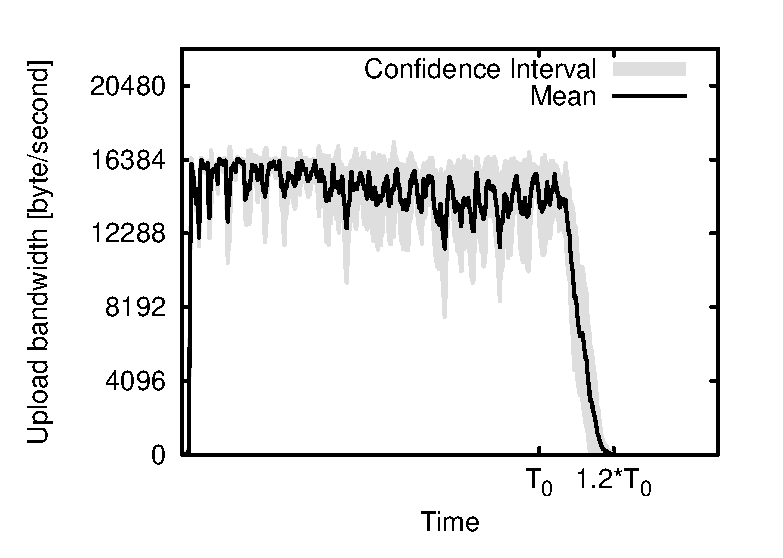
\includegraphics[width=0.49\textwidth]{fig/plots/scenario_6_parts_20/plots/GeneratedMeanCurrentUploadBandwidth.csv.eps}
    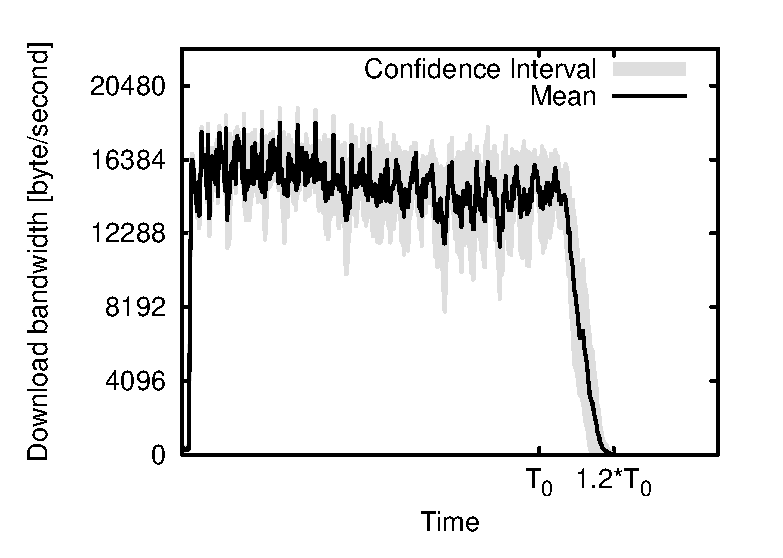
\includegraphics[width=0.49\textwidth]{fig/plots/scenario_6_parts_20/plots/GeneratedMeanCurrentDownloadBandwidth.csv.eps}
  \end{center}
\end{frame}


\begin{frame}
  \frametitle{Default Szenario mit 20 Datensätzen - Super-Peer Upload}
  \begin{center}
    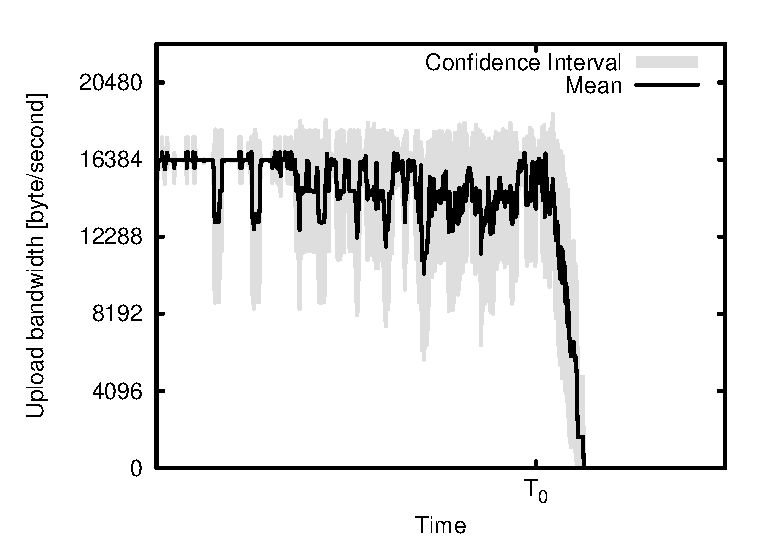
\includegraphics[width=0.49\textwidth]{fig/plots/scenario_6_parts_20/plots/GeneratedMeanCurrentSuperSeederUploadBandwidth.csv.eps}
  \end{center}
\end{frame}


%%%
%%% Fazit
%%%

\begin{frame}
  \frametitle{Fazit}
  
  \begin{block}{Einstellungen}
	  \begin{itemize}  
	    \item Gesamtdauer für Chunked-Swarm liegt unter $2*T_0$
	    \vspace{2mm}
	    \item Anzahl der Peers muss bekannt sein
	    \vspace{2mm}
	    \item Anzahl an Verbindungen wächst quadratisch: Skaliert nicht endlos
	    \vspace{2mm}
	    \item Einteilung in Sub-Datensätze ermöglicht Streaming
	  \end{itemize}		
  \end{block}
\end{frame}

%%%
%%% Future Work
%%%

\begin{frame}
  \frametitle{Future Work}
  \begin{itemize}
	  \item Simulationszeit: Hohe CPU Auslastung soll Messung nicht beeinflussen
	  \vspace{1mm}
	  \item Push-Based: Announcements wären nicht mehr nötig
	  \vspace{1mm}
	  \item Hierarchische Struktur: Verhindert quadratisches Wachstum an Verbindungen
  \end{itemize}		
\end{frame}


  \appendix

  
\section{Anhang}

\begin{frame}
  \frametitle{BitTorrent Live Paper}
  Clubbing with the Peers: A Measurement Study of BitTorrent Live
\end{frame}

%%%
%%% SCENARIO Seq
%%%

\begin{frame}
  \frametitle{Szenario Client\,/\,Server}
  \begin{block}{Einstellungen}
    \begin{itemize}  
      \item 1 Super-Peer und 63 Peers
      \vspace{2mm}
      \item Peers sind untereinander nicht verbunden
      \vspace{2mm}
      \item Anzahl der Chunks spielt keine Rolle
      \vspace{2mm}
      \item Datengröße so gewählt, dass $T_0=10$ Minuten gilt.
    \end{itemize}   
  \end{block}
\end{frame}

\begin{frame}
  \frametitle{Szenario Client\,/\,Server - Completion}
  \begin{center}
    \includegraphics[width=0.49\textwidth]{fig/plots/scenario_2_seq/plots/GeneratedMeanChunkCompletion.csv.eps}
    \hfill
    \includegraphics[width=0.49\textwidth]{fig/plots/scenario_2_seq/plots/GeneratedMeanSortedChunkCompletion.csv.eps}
  \end{center}
\end{frame}


\begin{frame}
  \frametitle{Szenario Client\,/\,Server - Upload/Download}
    \begin{itemize}  
    \item Links: Uploadbandbreite des Super-Peers
    \item Rechts: Downloadbandbreite der Peers
  \end{itemize}
  \begin{center}
    \includegraphics[width=0.49\textwidth]{fig/plots/scenario_2_seq/plots/GeneratedMeanCurrentSuperSeederUploadBandwidth.csv.eps}
    \includegraphics[width=0.49\textwidth]{fig/plots/scenario_2_seq/plots/GeneratedMeanCurrentDownloadBandwidth.csv.eps}
  \end{center}
\end{frame}


%%%
%%% Szenario Log
%%%

\begin{frame}
  \frametitle{Szenario Logarithmic}
  \begin{block}{Einstellungen}
    \begin{itemize}  
      \item 1 Super-Peer und 63 Peers
      \vspace{2mm}
      \item Peers (auch Super-Peer) senden gleichzeitig an max. einen Peer
      \vspace{2mm}
      \item Datensatz wird vollständig übertragen (kein Chunking)
      \vspace{2mm}
      \item Anzahl sendender Peers wächst exponentiell
      \vspace{2mm}
      \item Datengröße so gewählt, dass $T_0=10$ Minuten gilt.
    \end{itemize}   
  \end{block}
\end{frame}

\begin{frame}
  \frametitle{Szenario Logarithmic - Completion}
  \begin{center}
    \includegraphics[width=0.49\textwidth]{fig/plots/scenario_3_log/plots/GeneratedMeanChunkCompletion.csv.eps}
    \hfill
    \includegraphics[width=0.49\textwidth]{fig/plots/scenario_3_log/plots/GeneratedMeanSortedChunkCompletion.csv.eps}
  \end{center}
\end{frame}


\begin{frame}
  \frametitle{Szenario Logarithmic - Upload/Download}
  \begin{center}
    \includegraphics[width=0.49\textwidth]{fig/plots/scenario_3_log/plots/GeneratedMeanCurrentUploadBandwidth.csv.eps}
    \includegraphics[width=0.49\textwidth]{fig/plots/scenario_3_log/plots/GeneratedMeanCurrentDownloadBandwidth.csv.eps}
  \end{center}
\end{frame}


\begin{frame}
  \frametitle{Szenario Logarithmic - Super-Peer Upload}
  \begin{center}
    \includegraphics[width=0.49\textwidth]{fig/plots/scenario_3_log/plots/GeneratedMeanCurrentSuperSeederUploadBandwidth.csv.eps}
  \end{center}
\end{frame}


%%%
%%% SCENARIO 192
%%%

\begin{frame}
  \frametitle{Default Szenario mit 192 Peers - Completion}
  \begin{center}
    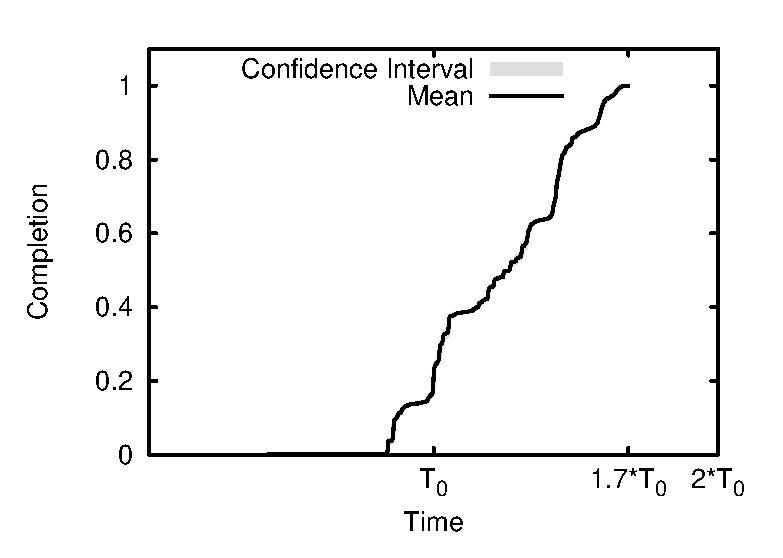
\includegraphics[width=0.49\textwidth]{fig/plots/scenario_11_peer_count_192_v2/plots/GeneratedMeanChunkCompletion.csv.eps}
    \hfill
    \includegraphics[width=0.49\textwidth]{fig/plots/scenario_11_peer_count_192_v2/plots/GeneratedMeanSortedChunkCompletion.csv.eps}
  \end{center}
\end{frame}


\begin{frame}
  \frametitle{Default Szenario mit 192 Peers - Upload/Download}
  \begin{center}
    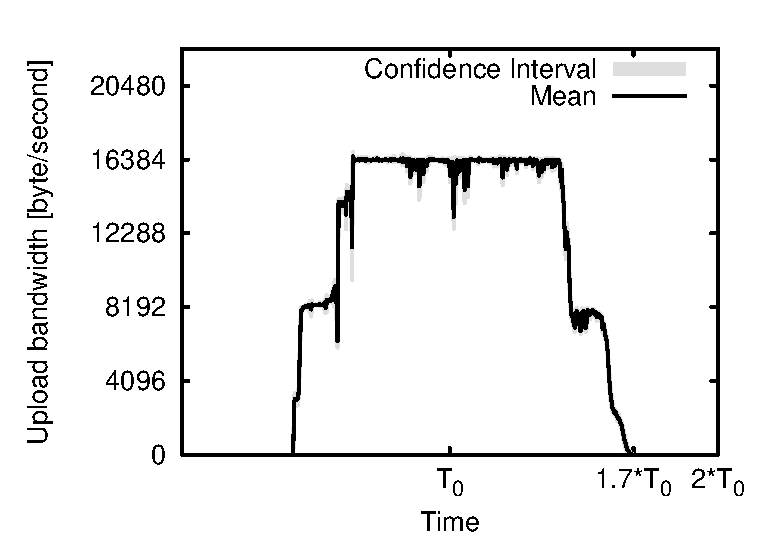
\includegraphics[width=0.49\textwidth]{fig/plots/scenario_11_peer_count_192_v2/plots/GeneratedMeanCurrentUploadBandwidth.csv.eps}
    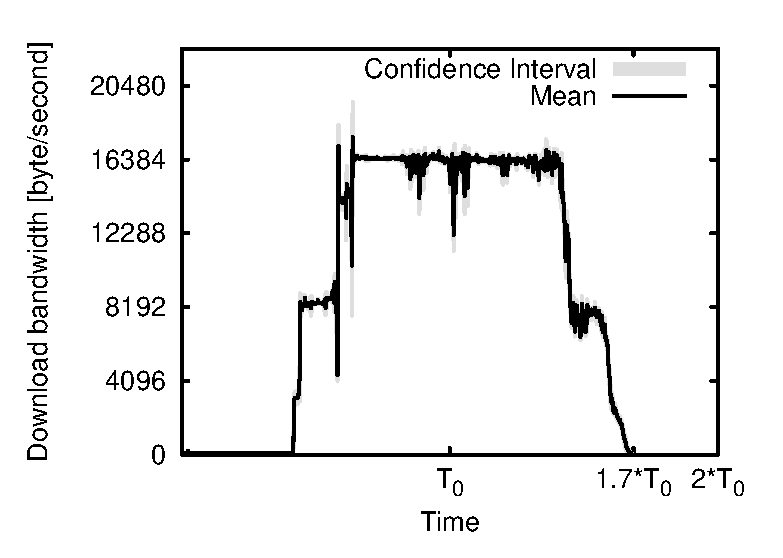
\includegraphics[width=0.49\textwidth]{fig/plots/scenario_11_peer_count_192_v2/plots/GeneratedMeanCurrentDownloadBandwidth.csv.eps}
  \end{center}
\end{frame}


\begin{frame}
  \frametitle{Default Szenario mit 192 Peers - Super-Peer Upload}
  \begin{center}
    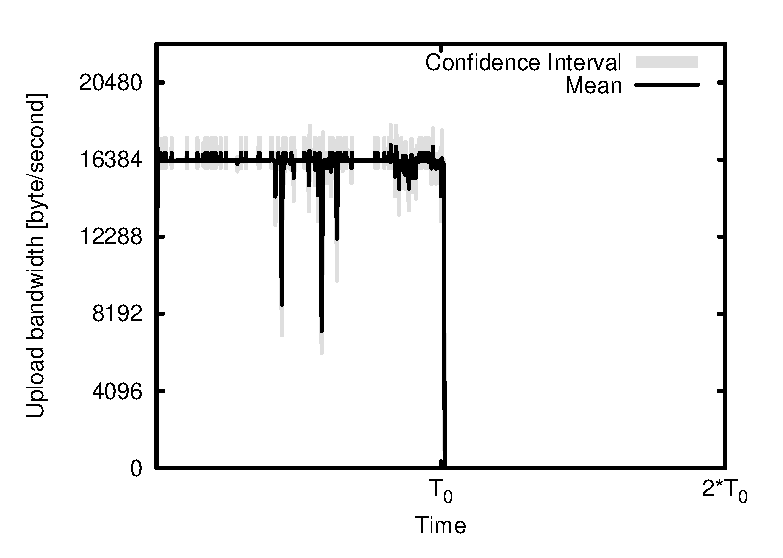
\includegraphics[width=0.49\textwidth]{fig/plots/scenario_11_peer_count_192_v2/plots/GeneratedMeanCurrentSuperSeederUploadBandwidth.csv.eps}
  \end{center}
\end{frame}


%%%
%%% Szenario MetaData 0
%%%

\begin{frame}
  \frametitle{Default Szenario mit Meta-Daten 0 - Completion}
  \begin{center}
    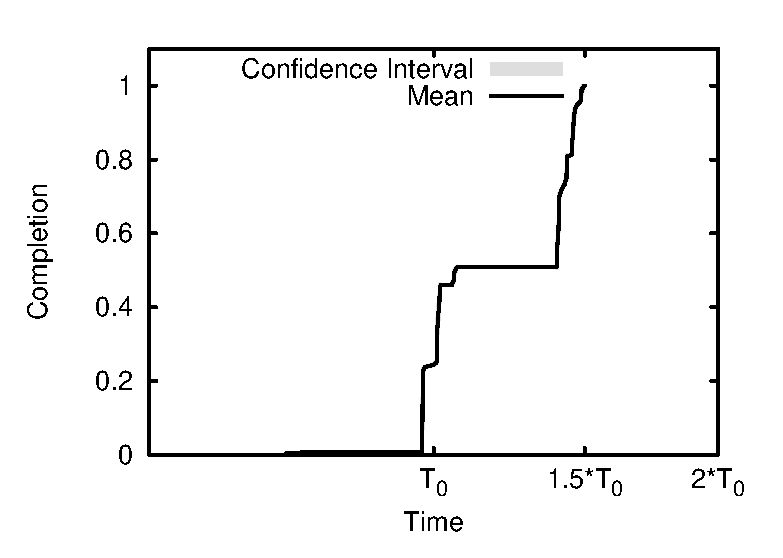
\includegraphics[width=0.49\textwidth]{fig/plots/scenario_5_meta_data_0/plots/GeneratedMeanChunkCompletion.csv.eps}
    \hfill
    \includegraphics[width=0.49\textwidth]{fig/plots/scenario_5_meta_data_0/plots/GeneratedMeanSortedChunkCompletion.csv.eps}
  \end{center}
\end{frame}


\begin{frame}
  \frametitle{Default Szenario mit Meta-Daten 0 - Upload/Download}
  \begin{center}
    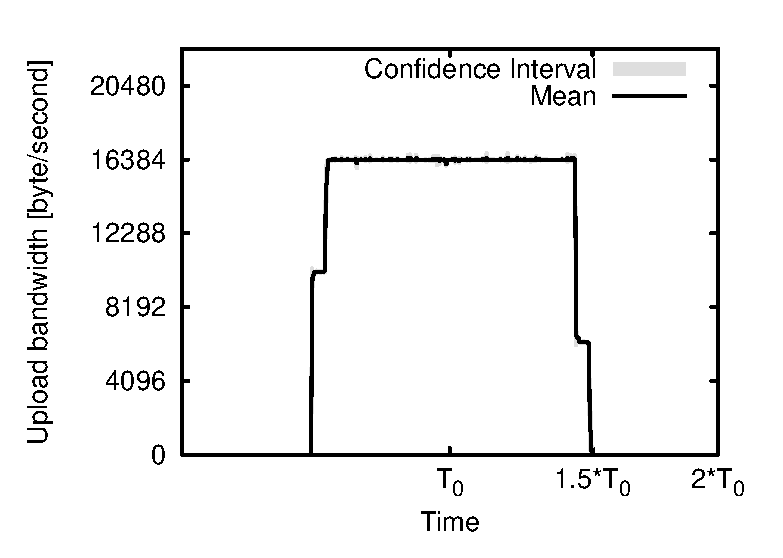
\includegraphics[width=0.49\textwidth]{fig/plots/scenario_5_meta_data_0/plots/GeneratedMeanCurrentUploadBandwidth.csv.eps}
    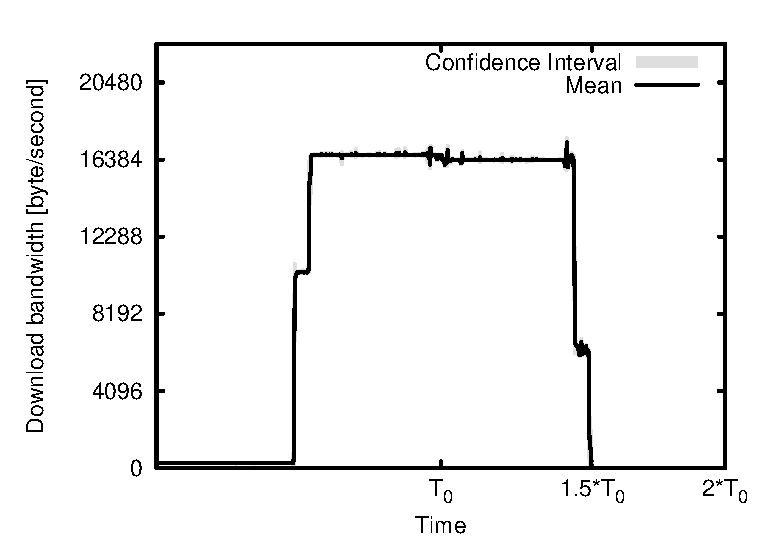
\includegraphics[width=0.49\textwidth]{fig/plots/scenario_5_meta_data_0/plots/GeneratedMeanCurrentDownloadBandwidth.csv.eps}
  \end{center}
\end{frame}


\begin{frame}
  \frametitle{Default Szenario mit Meta-Daten 0 - Super-Peer Upload}
  \begin{center}
    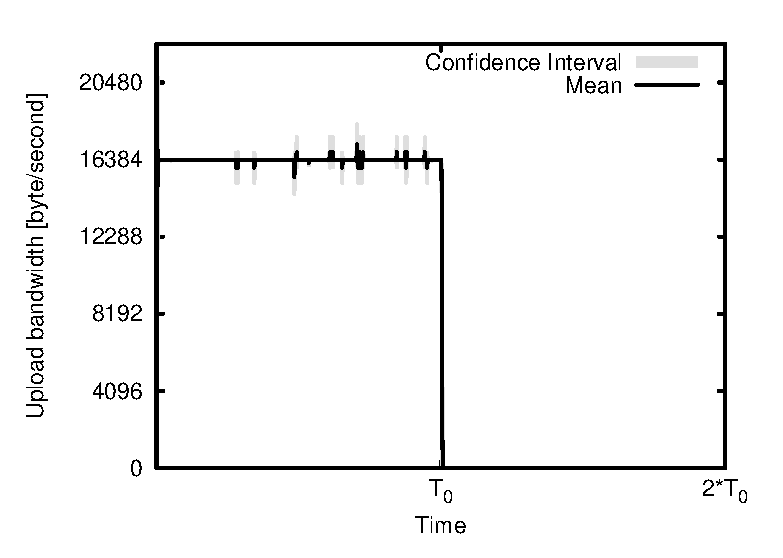
\includegraphics[width=0.49\textwidth]{fig/plots/scenario_5_meta_data_0/plots/GeneratedMeanCurrentSuperSeederUploadBandwidth.csv.eps}
  \end{center}
\end{frame}



%%%
%%% Szenario MetaData 10
%%%

\begin{frame}
  \frametitle{Default Szenario mit Meta-Daten 10 - Completion}
  \begin{center}
    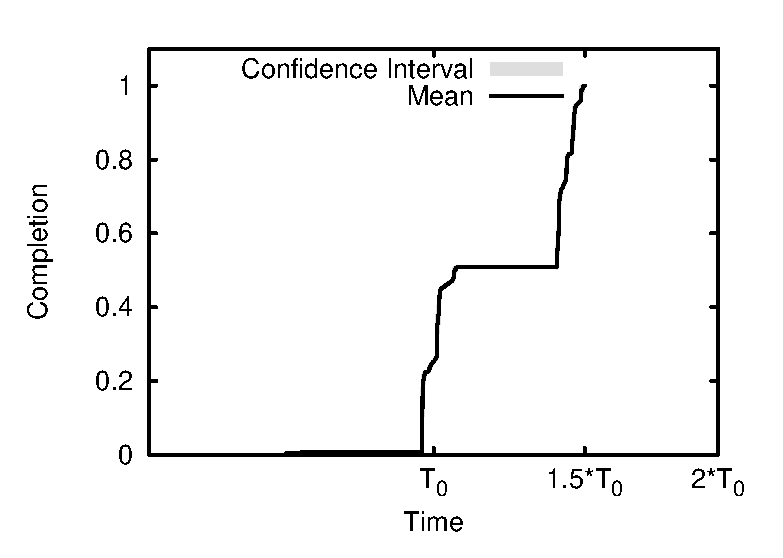
\includegraphics[width=0.49\textwidth]{fig/plots/scenario_10_meta_data_10/plots/GeneratedMeanChunkCompletion.csv.eps}
    \hfill
    \includegraphics[width=0.49\textwidth]{fig/plots/scenario_10_meta_data_10/plots/GeneratedMeanSortedChunkCompletion.csv.eps}
  \end{center}
\end{frame}


\begin{frame}
  \frametitle{Default Szenario mit Meta-Daten 10 - Upload/Download}
  \begin{center}
    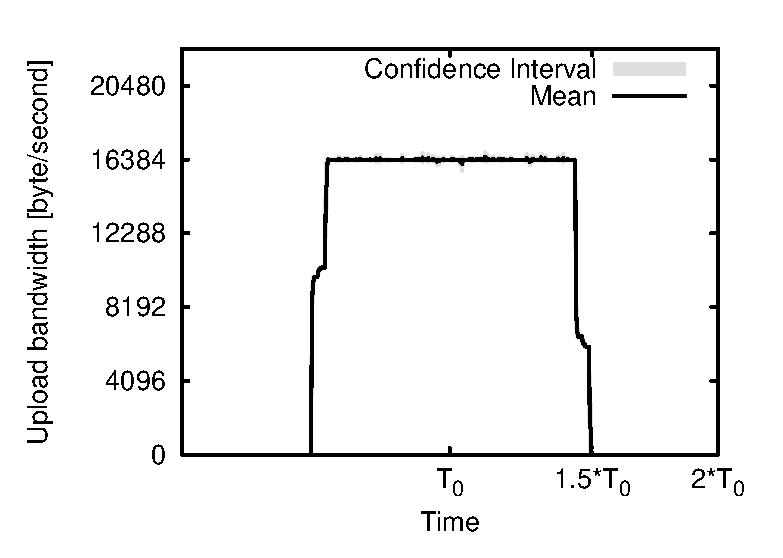
\includegraphics[width=0.49\textwidth]{fig/plots/scenario_10_meta_data_10/plots/GeneratedMeanCurrentUploadBandwidth.csv.eps}
    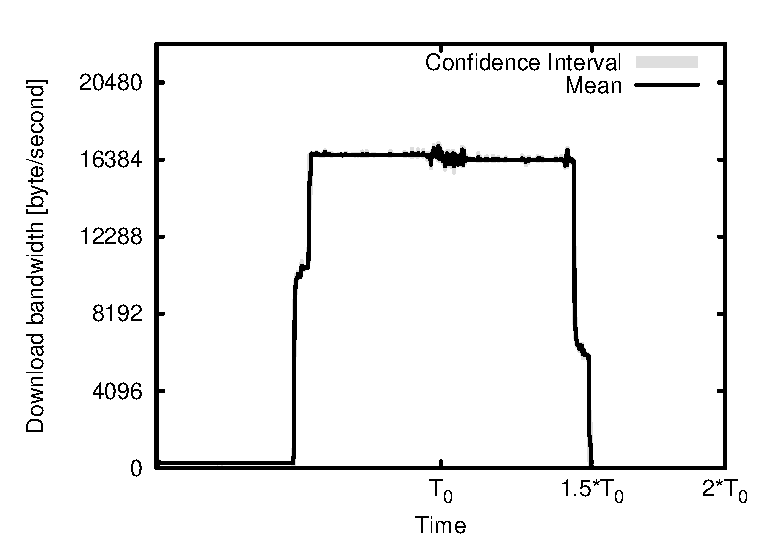
\includegraphics[width=0.49\textwidth]{fig/plots/scenario_10_meta_data_10/plots/GeneratedMeanCurrentDownloadBandwidth.csv.eps}
  \end{center}
\end{frame}


\begin{frame}
  \frametitle{Default Szenario mit Meta-Daten 10 - Super-Peer Upload}
  \begin{center}
    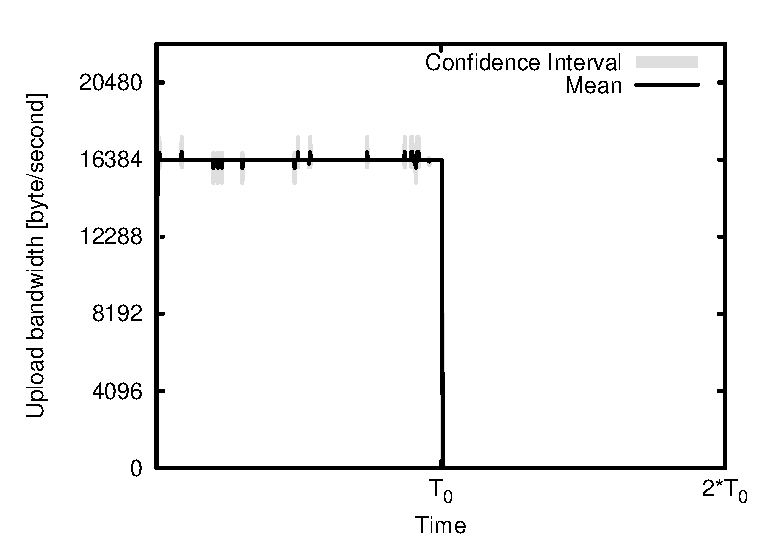
\includegraphics[width=0.49\textwidth]{fig/plots/scenario_10_meta_data_10/plots/GeneratedMeanCurrentSuperSeederUploadBandwidth.csv.eps}
  \end{center}
\end{frame}

%%%
%%% Szenario ChunkFac 1
%%%

\begin{frame}
  \frametitle{Default Szenario mit 1x Chunkanzahl - Completion}
  \begin{center}
    \includegraphics[width=0.49\textwidth]{fig/plots/scenario_7_chunk_count_fac_1/plots/GeneratedMeanChunkCompletion.csv.eps}
    \hfill
    \includegraphics[width=0.49\textwidth]{fig/plots/scenario_7_chunk_count_fac_1/plots/GeneratedMeanSortedChunkCompletion.csv.eps}
  \end{center}
\end{frame}


\begin{frame}
  \frametitle{Default Szenario mit 1x Chunkanzahl - Upload/Download}
  \begin{center}
    \includegraphics[width=0.49\textwidth]{fig/plots/scenario_7_chunk_count_fac_1/plots/GeneratedMeanCurrentUploadBandwidth.csv.eps}
    \includegraphics[width=0.49\textwidth]{fig/plots/scenario_7_chunk_count_fac_1/plots/GeneratedMeanCurrentDownloadBandwidth.csv.eps}
  \end{center}
\end{frame}


\begin{frame}
  \frametitle{Default Szenario mit 1x Chunkanzahl - Super-Peer Upload}
  \begin{center}
    \includegraphics[width=0.49\textwidth]{fig/plots/scenario_7_chunk_count_fac_1/plots/GeneratedMeanCurrentSuperSeederUploadBandwidth.csv.eps}
  \end{center}
\end{frame}

%%%
%%% Szenario ChunkFac 8
%%%

\begin{frame}
  \frametitle{Default Szenario mit 8x Chunkanzahl - Completion}
  \begin{center}
    \includegraphics[width=0.49\textwidth]{fig/plots/scenario_16_chunk_count_fac_8/plots/GeneratedMeanChunkCompletion.csv.eps}
    \hfill
    \includegraphics[width=0.49\textwidth]{fig/plots/scenario_16_chunk_count_fac_8/plots/GeneratedMeanSortedChunkCompletion.csv.eps}
  \end{center}
\end{frame}


\begin{frame}
  \frametitle{Default Szenario mit 8x Chunkanzahl - Upload/Download}
  \begin{center}
    \includegraphics[width=0.49\textwidth]{fig/plots/scenario_16_chunk_count_fac_8/plots/GeneratedMeanCurrentUploadBandwidth.csv.eps}
    \includegraphics[width=0.49\textwidth]{fig/plots/scenario_16_chunk_count_fac_8/plots/GeneratedMeanCurrentDownloadBandwidth.csv.eps}
  \end{center}
\end{frame}


\begin{frame}
  \frametitle{Default Szenario mit 8x Chunkanzahl - Super-Peer Upload}
  \begin{center}
    \includegraphics[width=0.49\textwidth]{fig/plots/scenario_16_chunk_count_fac_8/plots/GeneratedMeanCurrentSuperSeederUploadBandwidth.csv.eps}
  \end{center}
\end{frame}


%%%
%%% Szenario ChunkFac 16
%%%

\begin{frame}
  \frametitle{Default Szenario mit 16x Chunkanzahl - Completion}
  \begin{center}
    \includegraphics[width=0.49\textwidth]{fig/plots/scenario_17_chunk_count_fac_16/plots/GeneratedMeanChunkCompletion.csv.eps}
    \hfill
    \includegraphics[width=0.49\textwidth]{fig/plots/scenario_17_chunk_count_fac_16/plots/GeneratedMeanSortedChunkCompletion.csv.eps}
  \end{center}
\end{frame}


\begin{frame}
  \frametitle{Default Szenario mit 16x Chunkanzahl - Upload/Download}
  \begin{center}
    \includegraphics[width=0.49\textwidth]{fig/plots/scenario_17_chunk_count_fac_16/plots/GeneratedMeanCurrentUploadBandwidth.csv.eps}
    \includegraphics[width=0.49\textwidth]{fig/plots/scenario_17_chunk_count_fac_16/plots/GeneratedMeanCurrentDownloadBandwidth.csv.eps}
  \end{center}
\end{frame}


\begin{frame}
  \frametitle{Default Szenario mit 16x Chunkanzahl - Super-Peer Upload}
  \begin{center}
    \includegraphics[width=0.49\textwidth]{fig/plots/scenario_17_chunk_count_fac_16/plots/GeneratedMeanCurrentSuperSeederUploadBandwidth.csv.eps}
  \end{center}
\end{frame}


\end{document}


